\documentclass[aspectratio=169,10pt]{beamer}
\usetheme{metropolis}
\usepackage{amsmath,amssymb,braket}
\usepackage{tikz}
\usetikzlibrary{positioning,arrows.meta,shapes.geometric,calc,decorations.pathreplacing,fit,backgrounds}
\usepackage{xcolor}
\usepackage{listings}
\usepackage{appendixnumberbeamer}

% ── Color scheme ──
\definecolor{leangreen}{RGB}{34,180,34}
\definecolor{leanblue}{RGB}{70,130,180}
\definecolor{amber}{RGB}{255,191,0}
\definecolor{softred}{RGB}{220,80,80}
\definecolor{darkbg}{RGB}{15,15,15}
\definecolor{cardbg}{RGB}{30,30,30}
\definecolor{dimwhite}{RGB}{180,180,180}

\setbeamercolor{background canvas}{bg=darkbg}
\setbeamercolor{normal text}{fg=white}
\setbeamercolor{title}{fg=white}
\setbeamercolor{frametitle}{fg=white,bg=darkbg}
\setbeamercolor{block title}{fg=white,bg=gray!30!black}
\setbeamercolor{block body}{fg=white,bg=cardbg}
\setbeamercolor{alerted text}{fg=amber}
\setbeamercolor{example text}{fg=leangreen}
\setbeamercolor{itemize item}{fg=leangreen}
\setbeamercolor{itemize subitem}{fg=dimwhite}
\setbeamercolor{enumerate item}{fg=leangreen}
\setbeamercolor{progress bar}{fg=leangreen}
\setbeamercolor{title separator}{fg=leangreen}
\setbeamercolor{footline}{fg=dimwhite,bg=darkbg}

% ── Footer with page number / total ──
\setbeamertemplate{footline}{%
  \hfill%
  \usebeamercolor[fg]{footline}%
  \usebeamerfont{footline}%
  \insertframenumber\,/\,\inserttotalframenumber%
  \hspace*{6pt}\vspace{4pt}\par%
}

% ── Lean listing ──
\lstdefinelanguage{Lean}{
  keywords={theorem, lemma, def, abbrev, variable, namespace, end, open, import,
            noncomputable, private, section, structure, where, let, have, exact,
            intro, apply, simp, rw, rcases, refine, classical, cases, with,
            fun, forall, exists, Prop, Type},
  keywordstyle=\color{leanblue}\bfseries,
  keywords=[2]{IsInjective, SameMPV, GaugeEquiv, MPSTensor, Matrix, Fin, GL,
               CanonicalForm, AlgEquiv, TwoSidedIdeal},
  keywordstyle=[2]\color{leangreen},
  comment=[l]{--},
  commentstyle=\color{gray}\itshape,
  string=[b]",
  stringstyle=\color{orange},
  basicstyle=\ttfamily\scriptsize\color{white},
  backgroundcolor=\color{cardbg},
  breaklines=true,
  frame=single,
  rulecolor=\color{gray!50!black},
  showstringspaces=false,
  escapeinside={(*@}{@*)},
}
\lstset{language=Lean}

% ── Macros ──
\newcommand{\proved}[1]{\textcolor{leangreen}{\checkmark  #1}}
\newcommand{\inprog}[1]{\textcolor{amber}{$\circ$  #1}}
\newcommand{\future}[1]{\textcolor{gray}{$\diamond$  #1}}
\newcommand{\MD}{M_D(\mathbb{C})}
\newcommand{\GLC}{\mathrm{GL}}

\title{\textbf{Formalizing the Fundamental Theorem of\\Matrix Product States}}
\subtitle{{\small 2297 lines $\cdot$ 15 modules $\cdot$ 0 sorries\;\;$\cdot$\;\;Mathlib v4.27.0\;\;$\cdot$\;\;arXiv:2011.12127}}
\date{February 8, 2026}
\author{}

\begin{document}

%======================================================================
% SLIDE 1 - Title
%======================================================================
{%
\setbeamertemplate{footline}{}
\begin{frame}[plain,noframenumbering]
\vspace{-1em}
\maketitle
\end{frame}
}

%======================================================================
% SLIDE 2 - MPS Review
%======================================================================
\begin{frame}{Matrix Product States --- A 2-Minute Recap}
\begin{columns}[T]
\column{0.55\textwidth}
\textbf{Setup.} Physical index $i\in\{1,\dots,d\}$, bond dimension~$D$.\\[0.3em]
Assign a $D\times D$ matrix $A^i$ to each physical index.
\vspace{0.4em}

\textbf{The state} (periodic boundary conditions):
\begin{equation}
\ket{V^{(N)}} = \sum_{i_1,\dots,i_N} \mathrm{tr}\!(A^{i_1}\!\cdots A^{i_N}) \ket{i_1\cdots i_N}
\label{eq:mpv}
\end{equation}

\textbf{Gauge freedom.}
$B^i = X A^i X^{-1}$ with $X\in\GLC(D,\mathbb{C})$ leaves \emph{every} coefficient invariant by cyclicity of trace.

\textcolor{leangreen}{\textbf{[proved in GaugeInvariance.lean]}}

\column{0.43\textwidth}
\begin{center}
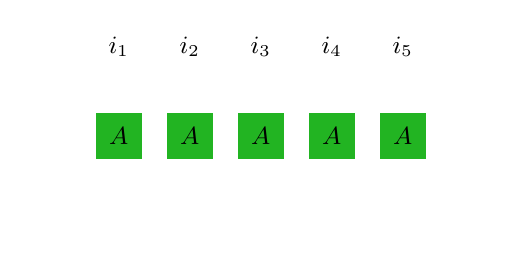
\begin{tikzpicture}[scale=0.82]
\foreach \x in {1,2,3,4,5} {
  \node[rectangle,draw=white,fill=leangreen,minimum size=0.6cm,
        font=\small\bfseries] (A\x) at (\x*1.1,0) {$A$};
  \draw[-,white,thick] (A\x.north) -- ++(0,0.55);
  \node[above=0.58cm of A\x,font=\small] {$i_{\x}$};
}
\foreach \x in {1,2,3,4} {
  \pgfmathtruncatemacro{\next}{\x+1}
  \draw[-,white,thick] (A\x.east) -- (A\next.west);
}
\draw[-,white,thick,densely dashed] (A1.west) -- ++(-0.5,0)
  node[left,font=\tiny] {tr};
\draw[-,white,thick,densely dashed] (A5.east) -- ++(0.5,0);
\draw[-,white,thick,densely dashed,rounded corners]
  ([xshift=-0.5cm]A1.west) -- ++(0,-0.7) -- ++(6.5,0) -- ++(0,0.7);
\node[font=\footnotesize\bfseries,white] at (3.3,-1.2) {bond dimension $D$};
\end{tikzpicture}

\vspace{1.5em}
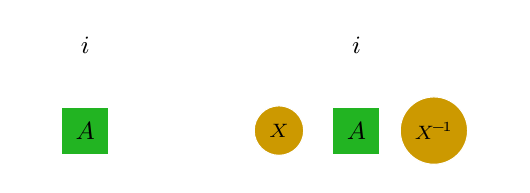
\begin{tikzpicture}[scale=0.82]
\node[rectangle,draw=white,fill=leangreen,minimum size=0.6cm,
      font=\small\bfseries] (Ai) at (0,0) {$A$};
\draw[-,white,thick] (Ai.north) -- ++(0,0.5);
\node[above=0.55cm of Ai,font=\small] {$i$};
\draw[-,white,thick] (Ai.west) -- ++(-0.5,0);
\draw[-,white,thick] (Ai.east) -- ++(0.5,0);
\node[font=\Large,white] at (2,0) {$=$};
\node[circle,draw=white,fill=amber!80!black,minimum size=0.55cm,
      font=\scriptsize\bfseries,text=black] (X) at (3,0) {$X$};
\node[rectangle,draw=white,fill=leangreen,minimum size=0.6cm,
      font=\small\bfseries] (A2) at (4.2,0) {$A$};
\node[circle,draw=white,fill=amber!80!black,minimum size=0.55cm,
      font=\scriptsize\bfseries,text=black] (Xi) at (5.4,0) {$X^{\!-\!1}$};
\draw[-,white,thick] (A2.north) -- ++(0,0.5);
\node[above=0.55cm of A2,font=\small] {$i$};
\draw[-,white,thick] (X.west) -- ++(-0.5,0);
\draw[-,white,thick] (X.east) -- (A2.west);
\draw[-,white,thick] (A2.east) -- (Xi.west);
\draw[-,white,thick] (Xi.east) -- ++(0.5,0);
\end{tikzpicture}
\end{center}
\end{columns}
\end{frame}

%======================================================================
% SLIDE 3 - The Fundamental Theorem
%======================================================================
\begin{frame}{The Fundamental Theorem of MPS}
\begin{block}{Theorem (Single-block, injective case) \hfill{\small [arXiv:2011.12127, Thm\,4.1]}}
Let $A=\{A^i\}_{i=1}^d$ be \textbf{injective}: the matrices $\{A^i\}$ span the full algebra $\MD$.

If tensors $A$ and $B$ generate the \textbf{same MPV family} for all system sizes $N$, then they are \textbf{gauge equivalent}:
\begin{equation}
B^i = X\, A^i\, X^{-1} \quad\text{for some } X\in\GLC(D,\mathbb{C})
\label{eq:gauge}
\end{equation}
\end{block}

\vspace{0.5em}
\textbf{Why does this matter?}
\begin{itemize}
\item \textbf{Classification of gapped phases:} gauge equivalence $\Leftrightarrow$ same phase
\item \textbf{SPT order:} symmetry action on gauge d.o.f.\ classifies SPT phases via $H^2(G,U(1))$
\item \textbf{Renormalization:} injective MPS are fixed points of the RG flow
\item \textbf{Parent Hamiltonians:} unique ground state iff injective --- gauge freedom is the \emph{only} ambiguity
\end{itemize}
\end{frame}

%======================================================================
% SLIDE 4 - Canonical Form
%======================================================================
\begin{frame}{The Full Picture: Canonical Form}
\begin{columns}[T]
\column{0.45\textwidth}
\begin{center}
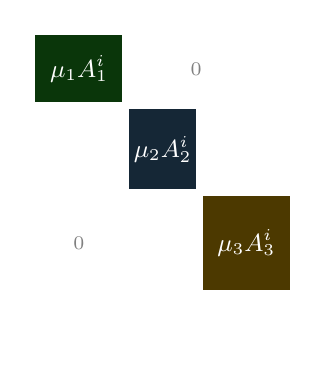
\begin{tikzpicture}[scale=0.85]
  \draw[white,thick] (0,0) rectangle (4,4);
  \fill[leangreen!30!black] (0.1,2.9) rectangle (1.4,3.9);
  \fill[leanblue!30!black] (1.5,1.6) rectangle (2.5,2.8);
  \fill[amber!30!black] (2.6,0.1) rectangle (3.9,1.5);
  \node[white,font=\small\bfseries] at (0.75,3.4) {$\mu_1 A_1^i$};
  \node[white,font=\small\bfseries] at (2.0,2.2) {$\mu_2 A_2^i$};
  \node[white,font=\small\bfseries] at (3.25,0.8) {$\mu_3 A_3^i$};
  \node[gray,font=\scriptsize] at (2.5,3.4) {$0$};
  \node[gray,font=\scriptsize] at (0.75,0.8) {$0$};
  \node[white,font=\bfseries] at (2,-0.5) {Block-diagonal};
\end{tikzpicture}
\end{center}

\column{0.52\textwidth}
Each block: $A_k^i$ injective, $\mu_k\in\mathbb{C}$ distinct.

\vspace{0.3em}
Block MPVs contribute independently:
\begin{equation}
V^{(N)} = \textstyle\sum_k \mu_k^N \cdot V_k^{(N)}
\label{eq:multiblock}
\end{equation}

\vspace{0.3em}
\textbf{Corollary 4.2:} Same state $\Rightarrow$ blocks match pairwise up to gauge + phase.

\vspace{0.5em}
\proved{Single-block theorem}\\
\proved{Multi-block decomposition}\\
\proved{Full corollary}
\end{columns}
\end{frame}

%======================================================================
% SLIDE 5 - Why Formalize?
%======================================================================
\begin{frame}{Why Formalize This Proof?}
\vspace{-0.3em}
\begin{columns}[T]
\column{0.48\textwidth}
{\small\textbf{\textcolor{softred}{The problem with physics proofs:}}}
\begin{itemize}\itemsep0.1em
\item {\small ``It is easy to see that\dots''}
\item {\small Index manipulations by hand}
\item {\small Implicit assumptions ($D>0$, fields algebraically closed, \dots)}
\item {\small Proofs build on each other --- errors propagate}
\end{itemize}

\vspace{0.3em}
{\small\textbf{This proof specifically:}}
\begin{itemize}\itemsep0.1em
\item {\small Uses deep algebra (Skolem--Noether!)}
\item {\small Requires careful handling of ring simplicity}
\item {\small SPT classification \emph{depends} on correctness}
\end{itemize}

\column{0.48\textwidth}
{\small\textbf{\textcolor{leangreen}{What formalization guarantees:}}}
\begin{itemize}\itemsep0.1em
\item {\small Every logical step machine-checked}
\item {\small All hypotheses made explicit}
\item {\small No ``exercise for the reader''}
\item {\small \textbf{0 sorries} = zero gaps}
\end{itemize}

\vspace{0.3em}
{\small\textbf{What we found:}}
\begin{itemize}\itemsep0.1em
\item {\small The paper proof is \emph{correct}}
\item {\small Many ``obvious'' steps are genuinely nontrivial}
\item {\small Precise hypotheses matter: $D>0$ needed in 6+ places}
\item {\small The algebraic bypass is essential}
\end{itemize}
\end{columns}
\end{frame}

%======================================================================
% SLIDE 6 - What is a Proof Assistant?
%======================================================================
\begin{frame}{What is a Proof Assistant?}
\begin{center}

\begin{tikzpicture}[
  box/.style={rectangle,rounded corners,draw=white,text=white,
              minimum width=3.2cm,minimum height=1.1cm,align=center,font=\small\bfseries},
  arr/.style={-{Stealth[scale=1.2]},white,thick}
]
\node[box,fill=leanblue!60!black] (input) at (0,0) {Definitions +\\Theorems +\\Proof scripts};
\node[box,fill=leangreen!40!black] (kernel) at (5.2,0) {Type-checking\\kernel\\{\footnotesize (tiny trusted core)}};
\node[box,fill=leangreen!60!black] (output) at (10.4,0) {\textcolor{leangreen}{\Large\checkmark}\\Proof verified};
\draw[arr] (input) -- (kernel);
\draw[arr] (kernel) -- (output);
\node[below=0.2cm of input,font=\footnotesize,text=dimwhite] {You write this};
\node[below=0.2cm of kernel,font=\footnotesize,text=dimwhite] {Computer checks};
\node[below=0.2cm of output,font=\footnotesize,text=dimwhite] {Guarantee};
\end{tikzpicture}
\end{center}

\vspace{0.3em}
{\small\textbf{Key analogy:} A proof assistant is a \emph{compiler for mathematics}.}
\begin{itemize}\itemsep0.05em
  \item {\small Compiler checks \emph{code} for type errors $ \longrightarrow $ Proof assistant checks \emph{proofs} for logical errors}
  \item {\small If it compiles, the proof is correct. Period.}
\end{itemize}

\vspace{0.2em}
{\small\textbf{What it is NOT:}}
\begin{itemize}\itemsep0.05em
  \item {\small Not computer algebra (Mathematica) --- those compute, not \emph{prove}}
  \item {\small Not automated theorem proving --- the human writes the proof, the machine \emph{verifies}}
  \item {\small Not just ``type-checking'' --- the type system encodes all of logic}
\end{itemize}
\end{frame}

%======================================================================
% SLIDE 7 - Lean 4 and Mathlib
%======================================================================
\begin{frame}{Lean 4 and Mathlib}
\vspace{-0.2em}
\begin{columns}[T]
\column{0.50\textwidth}
{\small\textbf{Lean 4} --- modern proof assistant (Microsoft Research, 2021+)}
\begin{itemize}\itemsep0.1em
  \item {\small Dependent type theory (CIC)}
  \item {\small Also a general-purpose programming language}
  \item {\small Fast, extensible, growing community}
\end{itemize}

\vspace{0.3em}
{\small\textbf{Mathlib} --- the mathematical library}
\begin{itemize}\itemsep0.1em
  \item {\small $>$\,1\,000\,000 lines of formalized math}
  \item {\small $\sim$700 contributors}
  \item {\small Covers: linear algebra, ring theory, topology, measure theory, \dots}
  \item {\small Crucially for us: \textbf{matrix algebras}, \textbf{simple rings}, \textbf{Skolem--Noether}}
\end{itemize}

\column{0.46\textwidth}
{\small\textbf{Recent successes:}}
\begin{itemize}\itemsep0.1em
  \item {\small\textbf{Liquid Tensor Experiment} (Scholze, 2022)}
  \item {\small\textbf{PFR Conjecture} (Tao et al., 2023)}
  \item {\small\textbf{Sphere eversion} (2023)}
\end{itemize}

\vspace{0.4em}
\begin{center}
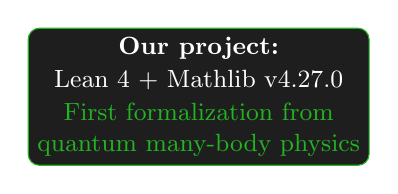
\begin{tikzpicture}
\node[rectangle,rounded corners,draw=leangreen,fill=cardbg,
      text=white,font=\small,align=center,
      minimum width=4.2cm,minimum height=1.3cm] {
  \textbf{Our project:}\\[0.1em]
  Lean 4 + Mathlib v4.27.0\\[0.1em]
  \textcolor{leangreen}{First formalization from}\\
  \textcolor{leangreen}{quantum many-body physics}
};
\end{tikzpicture}
\end{center}
\end{columns}
\end{frame}

%======================================================================
% SLIDE 8 - Zero Sorries
%======================================================================
\begin{frame}[fragile]{What Does ``0 Sorries'' Mean?}
In Lean, \texttt{sorry} is a magic axiom that closes \emph{any} goal:

\vspace{0.3em}
\begin{lstlisting}
theorem riemann_hypothesis : RiemannHypothesis := by
  sorry  -- accepted but flagged as incomplete!
\end{lstlisting}

\vspace{0.4em}
\begin{columns}[T]
\column{0.48\textwidth}
\textbf{\textcolor{softred}{With sorries:}}
\begin{itemize}
  \item Proof has gaps
  \item Like \texttt{// TODO} in code
  \item Lean warns: \textcolor{amber}{\texttt{uses sorry}}
\end{itemize}

\column{0.48\textwidth}
\textbf{\textcolor{leangreen}{With 0 sorries:}}
\begin{itemize}
  \item Every step verified by the kernel
  \item No gaps, no handwaving
  \item The proof is \emph{complete}
\end{itemize}
\end{columns}

\vspace{0.6em}
\begin{center}

\begin{tikzpicture}
\node[rectangle,rounded corners,draw=leangreen,fill=cardbg,
      text=white,minimum width=10cm,minimum height=0.9cm,
      align=center,font=\normalsize] {
\texttt{lake build}\ \textcolor{leangreen}{\checkmark}\quad
\textbf{Build successful --- 0 axioms, 0 sorries}
};
\end{tikzpicture}
\end{center}

\vspace{0.3em}
\textbf{Compare:} a typical proof says ``by a standard argument, $T$ is multiplicative.''  Our formalization: \textbf{159 lines} for multiplicativity alone.
\end{frame}

%======================================================================
% SLIDE 9 - The Challenge for Physics
%======================================================================
\begin{frame}{The Challenge: Formalizing Physics Proofs}
\begin{columns}[T]
\column{0.48\textwidth}
\begin{block}{\textcolor{softred}{Physics proof style}}
\begin{itemize}
\item ``It follows from the trace''
\item Implicit finite-dimensional
\item ``WLOG assume $D>0$''
\item Skip ``standard algebra''
\end{itemize}
\end{block}

\column{0.48\textwidth}
\begin{block}{\textcolor{leangreen}{Formal proof requires}}
\begin{itemize}
\item Every lemma cited explicitly
\item All types/dims declared
\item Case split on $D=0$ vs $D>0$
\item Prove or import from Mathlib
\end{itemize}
\end{block}
\end{columns}

\vspace{0.6em}
\textbf{The good news:} Mathlib already has an enormous library.
\begin{itemize}
  \item We get \textbf{Skolem--Noether}, \textbf{simplicity of $M_n(\mathbb{C})$}, \textbf{trace cyclicity}, \textbf{Vandermonde determinants} for free
  \item We had to \emph{build}: trace nondegeneracy, linear extension, multiplicativity, canonical form infrastructure
\end{itemize}

\vspace{0.3em}
\textbf{Expansion factor:} $\sim$3 pages of paper proof $ \longrightarrow $ 2297 lines of Lean $ \approx  10\times$ (typical)
\end{frame}

%======================================================================
% SLIDE 10 - Design Choices
%======================================================================
\begin{frame}[fragile]{Design Choices}
\textbf{Core type:}
\begin{lstlisting}
abbrev MPSTensor (d D : (*@$\mathbb{N}$@*)) := Fin d (*@$\to$@*) Matrix (Fin D) (Fin D) (*@$\mathbb{C}$@*)
\end{lstlisting}

\vspace{0.2em}
\begin{columns}[T]
\column{0.48\textwidth}
\textbf{Key definitions:}
\begin{lstlisting}
def IsInjective (A : MPSTensor d D) :=
  Submodule.span (*@$\mathbb{C}$@*) (Set.range A) = (*@$\top$@*)

def SameMPV (A B : MPSTensor d D) :=
  (*@$\forall$@*) N (*@$\sigma$@*), mpv A (*@$\sigma$@*) = mpv B (*@$\sigma$@*)

def GaugeEquiv (A B : MPSTensor d D) :=
  (*@$\exists$@*) X : GL (Fin D) (*@$\mathbb{C}$@*),
    (*@$\forall$@*) i, B i = X * A i * X(*@$^{-1}$@*)
\end{lstlisting}

\column{0.48\textwidth}
\textbf{Deliberate design decisions:}
\begin{itemize}
  \item \textbf{Algebraic injectivity:} $\{A^i\}$ span $\MD$\\
    {\small (avoids CP maps, Perron--Frobenius)}
  \item \textbf{$\GLC(D,\mathbb{C})$} for gauge transforms\\
    {\small (Mathlib's \texttt{GeneralLinearGroup})}
  \item \textbf{Sigma-type indices} for block-diagonal\\
    {\small (avoids painful \texttt{Fin} arithmetic)}
  \item \textbf{Word evaluation} via lists\\
    {\small (natural recursion)}
\end{itemize}
\end{columns}
\end{frame}

%======================================================================
% SLIDE 11 - Proof Strategy at a Glance
%======================================================================
\begin{frame}{Proof Strategy at a Glance}
\vspace{-0.4em}
\begin{center}
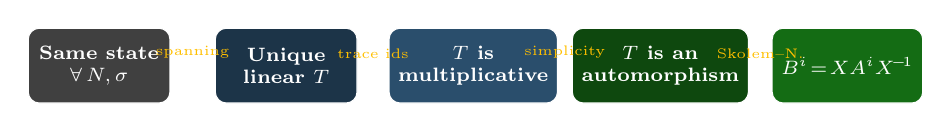
\begin{tikzpicture}[xscale=0.88,
  sbox/.style={rectangle,rounded corners,draw=white,text=white,
    font=\scriptsize\bfseries,minimum width=1.8cm,minimum height=0.95cm,align=center},
  sarr/.style={-{Stealth[scale=0.8]},white,thick},
  slab/.style={font=\tiny,text=amber,align=center,above,yshift=-1pt}
]
\node[sbox,fill=gray!50!black] (s0) at (0,0) {Same state\\$\forall\,N,\sigma$};
\node[sbox,fill=leanblue!40!black] (s1) at (2.7,0) {Unique\\linear $T$};
\node[sbox,fill=leanblue!60!black] (s2) at (5.4,0) {$T$ is\\multiplicative};
\node[sbox,fill=leangreen!40!black] (s3) at (8.1,0) {$T$ is an\\automorphism};
\node[sbox,fill=leangreen!60!black] (s4) at (10.8,0) {$B^i\!=\!XA^iX^{\!-\!1}$};
\draw[sarr] (s0) -- node[slab]{spanning} (s1);
\draw[sarr] (s1) -- node[slab]{trace ids} (s2);
\draw[sarr] (s2) -- node[slab]{simplicity} (s3);
\draw[sarr] (s3) -- node[slab]{Skolem--N.} (s4);
\end{tikzpicture}
\end{center}

\vspace{0.2em}
{\small\textbf{The argument in four sentences:}}
\begin{enumerate}\itemsep0.15em
  \item {\small \textbf{Same state $\boldsymbol{\Rightarrow}$ linear map.}
    Since $\{A^i\}$ span $\MD$, any linear map is determined by its values on $A^i$.
    SameMPV forces a \emph{unique} $T$ with $T(A^i)=B^i$.}
  \item {\small \textbf{Trace identities $\boldsymbol{\Rightarrow}$ multiplicativity.}
    SameMPV gives $\mathrm{tr}(A^iA^jA^k) = \mathrm{tr}(B^iB^jB^k)$.
    Injectivity of the trace pairing forces $T(MN)=T(M)\,T(N)$.}
  \item {\small \textbf{Simplicity $\boldsymbol{\Rightarrow}$ bijectivity.}
    $\ker T$ is a two-sided ideal of $M_D(\mathbb{C})$, which is simple.
    So $\ker T = 0$ and $T$ is an automorphism.}
  \item {\small \textbf{Skolem--Noether $\boldsymbol{\Rightarrow}$ conjugation.}
    Every automorphism of a matrix algebra is inner: $T(M) = XMX^{-1}$.
    Apply to each $A^i$.  Done!}
\end{enumerate}

\vspace{0.1em}
\begin{center}
{\small\textbf{Key:} Pure algebra --- traces, spanning, ring theory.\\No wavefunctions, no channels, no spectral theory.}
\end{center}
\end{frame}

%======================================================================
% SLIDE 12 - Step 1: Linear Extension
%======================================================================
\begin{frame}{Step 1: Linear Extension}
\textbf{Goal.} Since $\{A^i\}$ span $\MD$, there is a \emph{unique} linear map $T$ with $T(A^i) = B^i$.

\vspace{0.4em}
\begin{center}
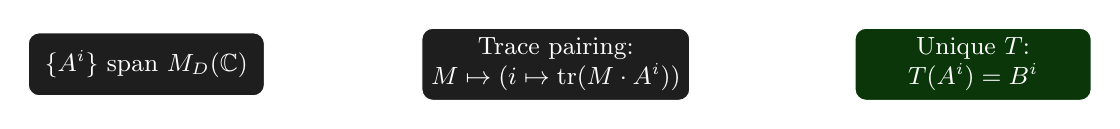
\begin{tikzpicture}[
  box/.style={rectangle,rounded corners,draw=white,fill=cardbg,text=white,
              minimum width=3cm,minimum height=0.8cm,align=center,font=\small}
]
\node[box] (span) at (0,0) {$\{A^i\}$ span $\MD$};
\node[box] (trace) at (5.2,0) {Trace pairing:\\$M\mapsto (i\mapsto \mathrm{tr}(M\cdot A^i))$};
\node[box,fill=leangreen!30!black] (ext) at (10.5,0) {Unique $T$:\\$T(A^i) = B^i$};
\draw[-{Stealth},white,thick] (span) -- node[above,font=\scriptsize]{injectivity} (trace);
\draw[-{Stealth},white,thick] (trace) -- node[above,font=\scriptsize]{left inverse} (ext);
\end{tikzpicture}
\end{center}

\vspace{0.4em}
\textbf{Key ingredients:}
\begin{itemize}
  \item Trace pairing $\Phi_A: M \mapsto (i\mapsto \mathrm{tr}(M\cdot A^i))$ is injective when $A$ is injective
  \item $\mathrm{SameMPV} \Rightarrow$ Gram compatibility: $\Phi_A \circ \mathrm{lc}_A = \Phi_B \circ \mathrm{lc}_B$
  \item Range inclusion + finrank argument $\Rightarrow$ $\Phi_B$ also injective
  \item $T = \Phi_B^{-1}\circ \Phi_A$ is the unique extension
\end{itemize}

\vspace{0.3em}
\textcolor{leangreen}{\checkmark}  \texttt{linearExtension\_exists\_unique} --- 88 lines
\end{frame}

%======================================================================
% SLIDE 12 - Step 2: Multiplicativity
%======================================================================
\begin{frame}{Step 2: Multiplicativity --- The Key Step}
\textbf{Goal.} Show $T(MN) = T(M)\,T(N)$ for all $M,N\in\MD$.

\vspace{0.4em}
\textbf{Strategy:} Trace identities from SameMPV, then extend by spanning.
\begin{enumerate}
  \item \textbf{Length-2 traces:}  $\mathrm{tr}(A^i A^j) = \mathrm{tr}(B^i B^j)$ \hfill {\small from SameMPV}
  \item \textbf{Compatibility:}  $\Phi_B \circ T = \Phi_A$ on generators, hence everywhere \hfill {\small by spanning}
  \item \textbf{Length-3 traces:}  $\mathrm{tr}(A^i A^j A^k) = \mathrm{tr}(B^i B^j B^k)$ \hfill {\small from SameMPV}
  \item \textbf{Injectivity of $\Phi_B$:}  Conclude $T(A^i \cdot A^j) = B^i B^j$ \hfill {\small inject into $\Phi_B$}
  \item \textbf{Bilinear extension:}  $\{A^i\}$ span $\Rightarrow$ $T(MN)=T(M)T(N)$ \hfill {\small two rounds}
\end{enumerate}

\vspace{0.4em}
\begin{block}{The crucial lemma underneath}
\textbf{Trace nondegeneracy:}  $\mathrm{tr}(MN)=0 \forall N \Longrightarrow  M=0$\quad {\small (31 lines, via single-entry matrices)}
\end{block}

\vspace{0.3em}
\textcolor{leangreen}{\checkmark}  \texttt{linearExtension\_mul} --- 54 lines
\end{frame}

%======================================================================
% SLIDE 13 - Step 3: Simplicity
%======================================================================
\begin{frame}{Step 3: Simplicity $\Rightarrow$ Bijectivity}
\vspace{-0.2em}
{\small\textbf{Have:} $T:\MD\to\MD$ is a nonzero multiplicative linear map.
\quad\textbf{Want:} $T$ is bijective (hence an algebra automorphism).}

\vspace{0.3em}
\begin{center}
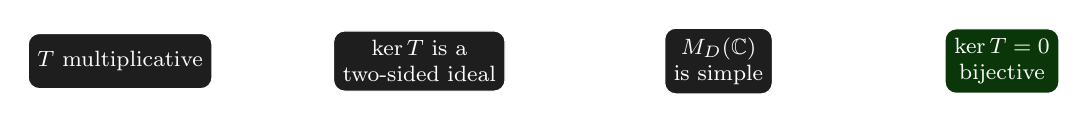
\begin{tikzpicture}[
  box/.style={rectangle,rounded corners,draw=white,fill=cardbg,text=white,
              minimum height=0.7cm,align=center,font=\footnotesize},
  arr/.style={-{Stealth[scale=1.0]},white,thick}
]
\node[box] (mult) at (0,0) {$T$ multiplicative};
\node[box] (ring) at (3.8,0) {$\ker T$ is a\\two-sided ideal};
\node[box] (simple) at (7.6,0) {$M_D(\mathbb{C})$\\is simple};
\node[box,fill=leangreen!30!black] (conc) at (11.2,0) {$\ker T = 0$\\bijective};
\draw[arr] (mult) -- (ring);
\draw[arr] (ring) -- (simple);
\draw[arr] (simple) -- (conc);
\end{tikzpicture}
\end{center}

\vspace{0.2em}
\begin{itemize}\itemsep0.05em
  \item {\small $T$ multiplicative $\Rightarrow$ $\ker T$ is a two-sided ideal of $\MD$}
  \item {\small $\MD$ is \textbf{simple} (no nontrivial two-sided ideals) \hfill \textcolor{leanblue}{[Mathlib]}}
  \item {\small $\ker T \in \{0, \MD\}$; since $T\neq 0$, we get $\ker T = 0$}
  \item {\small Injective + finite-dim $\Rightarrow$ surjective $\Rightarrow$ bijective}
\end{itemize}

\vspace{0.2em}
{\small\textbf{$T\neq 0$ proof:}  If $T=0$ then $B^i=0$, so $\mathrm{tr}(A^i)=0$ for all $i$. Since $\{A^i\}$ span, trace vanishes everywhere --- but $\mathrm{tr}(\mathbf{1}) = D \neq 0$.}

\vspace{0.15em}
{\small\textcolor{leangreen}{\checkmark}  \texttt{linear\_mul\_endomorphism\_bijective} --- uses \texttt{TwoSidedIdeal.ker}, \texttt{IsSimpleRing}}
\end{frame}

%======================================================================
% SLIDE 14 - Step 4: Skolem--Noether
%======================================================================
\begin{frame}[fragile]{Step 4: Skolem--Noether --- The Deep Theorem}
\vspace{-0.5em}
\begin{block}{Skolem--Noether Theorem}
{\small Every $\mathbb{C}$-algebra automorphism of $M_n(\mathbb{C})$ is \textbf{inner}: $ T(M) = X M X^{-1}$.}
\end{block}
\vspace{-0.1em}
{\small In Mathlib:}
\begin{lstlisting}[basicstyle=\ttfamily\scriptsize\color{white}]
-- Mathlib: every automorphism of End(V) is conjugation
AlgEquiv.eq_linearEquivConjAlgEquiv
\end{lstlisting}
\vspace{-0.1em}
{\small\textbf{Our bridge} (152 lines in \texttt{SkolemNoether.lean}):}
\begin{enumerate}\itemsep0.02em
  \item {\small Promote $T$ to \texttt{AlgEquiv} (must prove $T(1)=1$ from surjectivity!)}
  \item {\small Transport to \texttt{Module.End} via $M_n(\mathbb{C}) \cong \mathrm{End}(\mathbb{C}^n)$}
  \item {\small Apply Mathlib's Skolem--Noether}
  \item {\small Convert \texttt{LinearEquiv} back to $X\in\GLC(D,\mathbb{C})$}
\end{enumerate}
\vspace{-0.1em}
{\small\textbf{Subtlety:} $T(1)=1$ is nontrivial! Pick $x$ with $T(x)=1$, then
$1 = T(x) = T(x\cdot 1) = T(x)\,T(1) = T(1)$.}

\vspace{0.1em}
{\small\textcolor{leangreen}{\checkmark}  \texttt{skolemNoether\_matrix} --- Mathlib does the heavy lifting}
\end{frame}

%======================================================================
% SLIDE 15 - Step 5: Assembly
%======================================================================
\begin{frame}[fragile]{Step 5: Assembly --- The Main Theorem}
\vspace{-0.8em}
\begin{lstlisting}[basicstyle=\ttfamily\fontsize{6}{7.5}\selectfont\color{white}]
theorem fundamentalTheorem_singleBlock
    {A B : MPSTensor d D}
    (hA : IsInjective A) (hAB : SameMPV A B) :
    GaugeEquiv A B := by
  classical
  cases D with
  | zero => exact (*@$\langle$@*)1, fun i => by simpa(*@$\rangle$@*)
  | succ D' =>
    -- 1. Linear extension
    rcases linearExtension_exists_unique hA hAB with (*@$\langle$@*)T, hT, -(*@$\rangle$@*)
    -- 2. Multiplicativity + nonzero => bijective
    have hMul := linearExtension_mul hA hAB hT
    have hBij := linear_mul_endomorphism_bijective T
                   hMul (linearExtension_nonzero hA hAB hT)
    -- 3. Skolem-Noether
    let fHom := linearMapToAlgHom T hMul hBij.surjective
    let f := AlgEquiv.ofBijective fHom hBij
    rcases skolemNoether_matrix f with (*@$\langle$@*)X, hX(*@$\rangle$@*)
    -- 4. Assemble: B i = T(A i) = X * A i * X^(-1)
    refine (*@$\langle$@*)X, fun i => ?_(*@$\rangle$@*)
    have hfi : f (A i) = B i := by simpa using hT i
    simpa [hfi] using hX (A i)
\end{lstlisting}
\vspace{-0.5em}
\begin{center}
{\small\textcolor{leangreen}{\checkmark}\;\textbf{78 lines total (FundamentalTheorem.lean)}\;\textcolor{leangreen}{\checkmark}}
\end{center}
\end{frame}

%======================================================================
% SLIDE 16 - Proof Flowchart
%======================================================================
\begin{frame}{The Complete Proof Pipeline}
\vspace{-0.3em}
\begin{center}
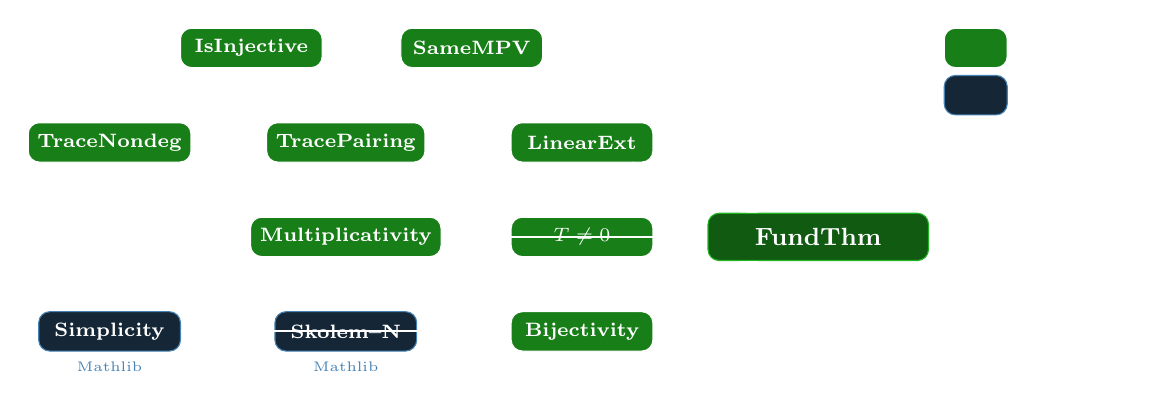
\begin{tikzpicture}[
  node distance=0.9cm and 0.6cm,
  lemma/.style={rectangle,draw=white,fill=leangreen!70!black,text=white,
        font=\scriptsize\bfseries,minimum width=1.8cm,minimum height=0.5cm,rounded corners},
  mathlib/.style={rectangle,draw=leanblue,fill=leanblue!30!black,text=white,
        font=\scriptsize\bfseries,minimum width=1.8cm,minimum height=0.5cm,rounded corners},
  main/.style={rectangle,draw=leangreen,fill=leangreen!50!black,text=white,
        font=\small\bfseries,minimum width=2.8cm,minimum height=0.6cm,rounded corners},
  arrow/.style={-{Stealth[scale=0.9]},white,thick}
]
\node[lemma] (inj) at (0,3.8) {IsInjective};
\node[lemma] (same) at (2.8,3.8) {SameMPV};
\node[lemma] (tracend) at (-1.8,2.6) {TraceNondeg};
\node[lemma] (tracep) at (1.2,2.6) {TracePairing};
\node[lemma] (linext) at (4.2,2.6) {LinearExt};
\node[lemma] (mult) at (1.2,1.4) {Multiplicativity};
\node[lemma] (nonzero) at (4.2,1.4) {$T\neq 0$};
\node[mathlib] (simple) at (-1.8,0.2) {Simplicity};
\node[below=0.01cm of simple,font=\tiny,text=leanblue] {Mathlib};
\node[mathlib] (sn) at (1.2,0.2) {Skolem--N};
\node[below=0.01cm of sn,font=\tiny,text=leanblue] {Mathlib};
\node[lemma] (bij) at (4.2,0.2) {Bijectivity};
\node[main] (thm) at (7.2,1.4) {\textbf{FundThm}};
\draw[arrow] (inj) -- (tracep);
\draw[arrow] (same) -- (tracep);
\draw[arrow] (same) -- (linext);
\draw[arrow] (inj) -- (linext);
\draw[arrow] (tracend) -- (tracep);
\draw[arrow] (tracep) -- (mult);
\draw[arrow] (tracep) -- (linext);
\draw[arrow] (linext) -- (thm);
\draw[arrow] (mult) -- (thm);
\draw[arrow] (nonzero) -- (bij);
\draw[arrow] (mult) -- (bij);
\draw[arrow] (simple) -- (bij);
\draw[arrow] (bij) -- (thm);
\draw[arrow] (sn) -- (thm);
% Legend — positioned within visible area
\node[lemma,minimum width=0.8cm,font=\tiny] (leg1) at (9.2,3.8) {};
\node[text=white,font=\scriptsize,right=0.15cm of leg1] {Our code};
\node[mathlib,minimum width=0.8cm,font=\tiny] (leg2) at (9.2,3.2) {};
\node[text=white,font=\scriptsize,right=0.15cm of leg2] {Mathlib};
\end{tikzpicture}
\end{center}
\end{frame}

%======================================================================
% SLIDE 17 - What Mathlib Gave Us
%======================================================================
\begin{frame}{What Mathlib Gave Us vs.\ What We Built}
\begin{columns}[T]
\column{0.48\textwidth}
\textbf{\textcolor{leanblue}{From Mathlib (free!):}}
\begin{itemize}
  \item[\textcolor{leanblue}{$\blacksquare$}] \texttt{IsSimpleRing} for $M_n(\mathbb{C})$
  \item[\textcolor{leanblue}{$\blacksquare$}] Skolem--Noether
  \item[\textcolor{leanblue}{$\blacksquare$}] Trace cyclicity, linearity
  \item[\textcolor{leanblue}{$\blacksquare$}] \texttt{blockDiagonal'}, block multiplication
  \item[\textcolor{leanblue}{$\blacksquare$}] Vandermonde determinant
  \item[\textcolor{leanblue}{$\blacksquare$}] $\GLC(D,\mathbb{C})$, rank--nullity
  \item[\textcolor{leanblue}{$\blacksquare$}] \texttt{Submodule.span}, \texttt{ext\_on\_range}
\end{itemize}

\column{0.48\textwidth}
\textbf{\textcolor{leangreen}{We had to build:}}
\begin{itemize}
  \item[\textcolor{leangreen}{$\blacksquare$}] Trace nondegeneracy (31 lines)
  \item[\textcolor{leangreen}{$\blacksquare$}] Trace pairing map $\Phi_A$ (99 lines)
  \item[\textcolor{leangreen}{$\blacksquare$}] Linear extension existence + uniqueness
  \item[\textcolor{leangreen}{$\blacksquare$}] Multiplicativity of $T$ (54 lines)
  \item[\textcolor{leangreen}{$\blacksquare$}] $T\neq 0$ argument, $T(1)=1$
  \item[\textcolor{leangreen}{$\blacksquare$}] Matrix $\leftrightarrow$ End transport
  \item[\textcolor{leangreen}{$\blacksquare$}] Canonical form, block MPV decomposition
  \item[\textcolor{leangreen}{$\blacksquare$}] Vandermonde separation for MPVs
\end{itemize}
\end{columns}
\end{frame}

%======================================================================
% SLIDE 18 - What We Avoided
%======================================================================
\begin{frame}{The Algebraic Bypass: What We Deliberately Avoided}
\begin{columns}[T]
\column{0.46\textwidth}
\begin{block}{\textcolor{softred}{Standard physics route}}
\begin{itemize}
\item CP maps / quantum channels
\item Perron--Frobenius theorem
\item Spectral radius of transfer operator
\item Fixed-point equations
\item Positivity arguments
\end{itemize}
\end{block}

\column{0.46\textwidth}
\begin{block}{\textcolor{leangreen}{Our algebraic route}}
\begin{itemize}
\item Spanning $\Rightarrow$ linear extension
\item Trace identities $\Rightarrow$ multiplicativity
\item Simple ring $\Rightarrow$ bijectivity
\item Skolem--Noether $\Rightarrow$ inner
\item Pure linear algebra!
\end{itemize}
\end{block}
\end{columns}

\vspace{0.5em}
\textbf{Why the bypass?}
\begin{itemize}
  \item Perron--Frobenius for CP maps is \textbf{not in Mathlib}
  \item The algebraic route uses only linear algebra + ring theory --- all well-covered
  \item Already noted in the paper: injective case doesn't need channel theory
  \item \textbf{Bonus:} the algebraic proof is arguably \emph{cleaner}
\end{itemize}
\end{frame}

%======================================================================
% SLIDE 19 - Canonical Form Structure
%======================================================================
\begin{frame}[fragile]{Multi-Block: The Canonical Form Structure}
\vspace{-0.3em}
\begin{lstlisting}[basicstyle=\ttfamily\footnotesize\color{white}]
structure CanonicalForm (d : (*@$\mathbb{N}$@*)) where
  numBlocks   : (*@$\mathbb{N}$@*)
  blockDim    : Fin numBlocks (*@$\to$@*) (*@$\mathbb{N}$@*)
  blockTensor : (k : Fin numBlocks) (*@$\to$@*) MPSTensor d (blockDim k)
  (*@$\mu$@*)           : Fin numBlocks (*@$\to$@*) (*@$\mathbb{C}$@*)
  block_injective : (*@$\forall$@*) k, IsInjective (blockTensor k)
\end{lstlisting}
\vspace{0.1em}
{\small\textbf{Assembly:}}
\begin{lstlisting}[basicstyle=\ttfamily\footnotesize\color{white}]
noncomputable def toTensor : MPSTensor d C.totalDim :=
  fun i => (Matrix.reindex e e)
    (Matrix.blockDiagonal' (fun k => C.(*@$\mu$@*) k (*@$\bullet$@*) C.blockTensor k i))
\end{lstlisting}
\vspace{0.1em}
{\small\textbf{Key design:} Block-diagonal on $\Sigma$-type indices
$\bigsqcup_k \mathrm{Fin}(D_k)$, then reindex to $\mathrm{Fin}(\sum_k D_k)$.}

{\small Uses Mathlib's \texttt{blockDiagonal'\_mul}, \texttt{trace\_blockDiagonal'} directly --- avoids all \texttt{Fin} sub-range arithmetic.}

\vspace{0.2em}
{\small\textcolor{leangreen}{\checkmark}  \texttt{CanonicalForm.lean} --- 52 lines}
\end{frame}

%======================================================================
% SLIDE 20 - Key Decomposition
%======================================================================
\begin{frame}{Multi-Block: The Workhorse Lemma}
\vspace{-0.3em}
\begin{block}{MPV Decomposition (\texttt{mpv\_toTensor\_eq\_sum})}
\vspace{-0.5em}
\begin{equation}
\mathrm{mpv}(\mathrm{toTensor}(C), \sigma) =  \sum_{k=1}^{r} \mu_k^N \cdot \mathrm{mpv}(A_k, \sigma)
\label{eq:decomp}
\end{equation}
\end{block}

\vspace{0.15em}
{\small\textbf{Proof outline} (285 lines in \texttt{MultiBlock.lean}):}
\begin{enumerate}\itemsep0.05em
  \item {\small\texttt{evalWord} of reindexed tensor $=$ reindex of \texttt{evalWord}}
  \item {\small\texttt{evalWord} of block-diagonal $=$ block-diagonal of block \texttt{evalWord}s}
  \item {\small With scaling: each block picks up $\mu_k^{|w|}$}
  \item {\small\texttt{trace\_reindex}: remove outer reindexing}
  \item {\small\texttt{trace\_blockDiagonal'}: split trace into sum}
  \item {\small Pull out scalar factors}
\end{enumerate}

\vspace{0.1em}
{\small This is the \textbf{computational backbone}: reduces multi-block questions to single-block questions weighted by powers of $\mu_k$.}

\vspace{0.1em}
{\small\textcolor{leangreen}{\checkmark}  \texttt{mpv\_toTensor\_eq\_sum} --- proved}
\end{frame}

%======================================================================
% SLIDE 21 - Vandermonde Separation
%======================================================================
\begin{frame}{Multi-Block: Vandermonde Separation}
\vspace{-0.5em}
{\small\textbf{Setup.} Two canonical forms give the same state:}
\vspace{-0.5em}
\[
\sum_k \mu_k^N \cdot V_k^{(N)}(\sigma) = \sum_j \nu_j^N \cdot W_j^{(N)}(\sigma) \qquad \forall  N, \sigma
\]
\vspace{-0.7em}

{\small\textbf{Key insight:} If $\{\mu_k\}$ are \emph{distinct}, this is a Vandermonde system!}

\vspace{0.1em}
\begin{columns}[T]
\column{0.55\textwidth}
{\small\textbf{Separation lemma:}\\
Distinct $\mu_k$ + $\sum_k c_k \mu_k^N = 0$ for $N=0,\dots,r{-}1$\\
$\Longrightarrow  c_k = 0 \forall k$}

\vspace{0.2em}
{\small Uses Mathlib's \texttt{det\_vandermonde}\\
and \texttt{eq\_zero\_of\_forall\_pow\_sum\_mul\_pow\_eq\_zero}.}

\vspace{0.2em}
{\small\textbf{Extended to MPVs:}\\
If block MPVs are nonzero and $\mu_k$ distinct, blocks can be separated.}

\column{0.40\textwidth}
\begin{center}
\begin{tikzpicture}[scale=0.6]
\draw[white,thick] (0,0) grid (3,3);
\foreach \j in {0,1,2} {
  \node[font=\tiny,white] at (\j+0.5,2.5) {$\mu_{\pgfmathparse{int(\j+1)}\pgfmathresult}^0$};
  \node[font=\tiny,white] at (\j+0.5,1.5) {$\mu_{\pgfmathparse{int(\j+1)}\pgfmathresult}^1$};
  \node[font=\tiny,white] at (\j+0.5,0.5) {$\mu_{\pgfmathparse{int(\j+1)}\pgfmathresult}^2$};
}
\node[below=0.15cm,white,font=\footnotesize\bfseries] at (1.5,0) {Vandermonde};
\node[below=0.45cm,white,font=\scriptsize] at (1.5,0) {$\det \neq 0$ iff $\mu_k$ distinct};
\end{tikzpicture}
\end{center}
\end{columns}

\vspace{0.1em}
{\small\textcolor{leangreen}{\checkmark}  \texttt{vandermonde\_separation}, \texttt{block\_mpvs\_lin\_indep\_at\_fixed\_size} --- 162 lines}
\end{frame}

%======================================================================
% SLIDE 22 - What's Next (Multi-Block)
%======================================================================
\begin{frame}{Multi-Block: What's Next}
\vspace{-0.3em}
\begin{center}
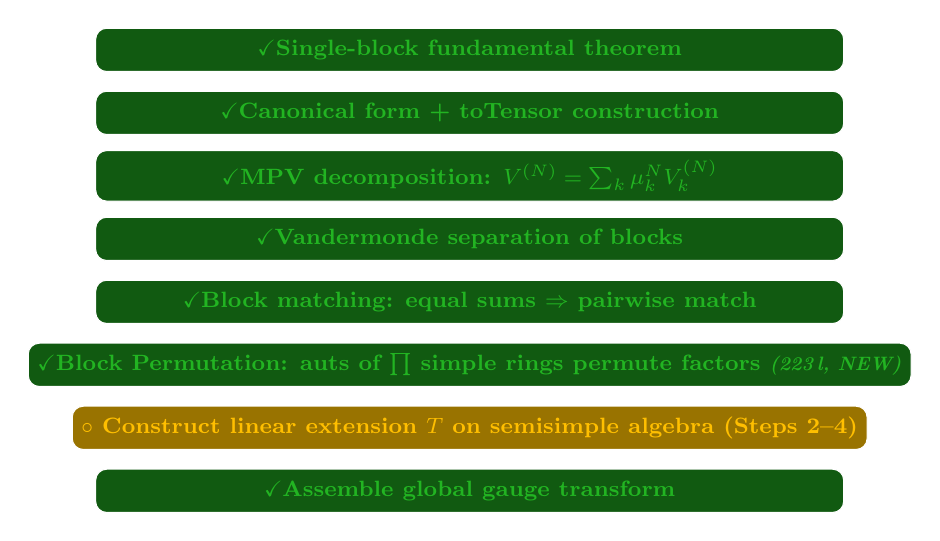
\begin{tikzpicture}[
  node distance=0.7cm,
  box/.style={rectangle,rounded corners,draw=white,text=white,
              font=\footnotesize\bfseries,minimum width=9.5cm,minimum height=0.55cm},
  done/.style={fill=leangreen!50!black},
  next/.style={fill=amber!60!black,text=black},
  fut/.style={fill=gray!40!black}
]
\node[box,done] (s1) at (0,3.6) {\proved{Single-block fundamental theorem}};
\node[box,done] (s2) at (0,2.8) {\proved{Canonical form + toTensor construction}};
\node[box,done] (s3) at (0,2.0) {\proved{MPV decomposition: $V^{(N)} = \sum_k \mu_k^N V_k^{(N)}$}};
\node[box,done] (s4) at (0,1.2) {\proved{Vandermonde separation of blocks}};
\node[box,done] (s5) at (0,0.4) {\proved{Block matching: equal sums $\Rightarrow$ pairwise match}};
\node[box,done] (s6) at (0,-0.4) {\proved{Block Permutation: auts of $\prod$ simple rings permute factors \emph{\scriptsize(223\,l, NEW)}}};
\node[box,next] (s7) at (0,-1.2) {\inprog{Construct linear extension $T$ on semisimple algebra (Steps 2--4)}};
\node[box,done] (s8) at (0,-2.0) {\proved{Assemble global gauge transform}};
\end{tikzpicture}
\end{center}

\vspace{0.15em}
{\small\textbf{New result --- Block Permutation Theorem:} automorphisms of $\prod_k M_{n_k}(\mathbb{C})$ must permute the simple factors.  Strategy: two-sided ideal classification $+$ atoms $+$ \texttt{OrderIso.isAtom\_iff}.}

\vspace{0.1em}
{\small\textbf{Remaining gap:} constructing the linear extension $T$ on the full semisimple algebra (the multi-block analogue of Steps 2--4).}
\end{frame}

%======================================================================
% SLIDE 23 - What We Can't Formalize (Yet)
%======================================================================
\begin{frame}{What We CAN'T Formalize (Yet)}
\vspace{-0.2em}
\begin{columns}[T]
\column{0.50\textwidth}
{\small\textbf{\textcolor{softred}{Not in Mathlib (yet):}}}
\begin{itemize}\itemsep0.1em
  \item {\small Perron--Frobenius for CP maps}
  \item {\small Spectral radius of transfer operator}
  \item {\small Quantum Wielandt (normality)}
  \item {\small Canonical form \emph{existence}}
\end{itemize}

\column{0.46\textwidth}
{\small\textbf{\textcolor{leangreen}{Our approach:}}}
\begin{itemize}\itemsep0.1em
  \item {\small Axiomatize canonical form as \texttt{structure}}
  \item {\small Assume injectivity of blocks}
  \item {\small Assume distinct $\mu_k$}
  \item {\small Prove everything \emph{downstream}}
\end{itemize}
\end{columns}

\vspace{0.4em}
{\small\textbf{This is sound:} we make hypotheses \emph{explicit}. The single-block theorem has \textbf{zero} axiomatization --- fully proven from Mathlib foundations.}

\vspace{0.3em}
{\small The formalization boundary is set by Mathlib's coverage of functional analysis, not by any fundamental limitation.}

\vspace{0.3em}
{\small\textbf{What would unlock the rest:}}
\begin{itemize}\itemsep0.05em
  \item {\small Perron--Frobenius for positive maps on $C^*$-algebras}
  \item {\small Spectral theory for finite-dim operators (partially in Mathlib)}
\end{itemize}
\end{frame}

%======================================================================
% SLIDE 24 - Lessons Learned
%======================================================================
\begin{frame}{Lessons Learned}
\begin{columns}[T]
\column{0.48\textwidth}
\textbf{\textcolor{leangreen}{Surprises (positive):}}
\begin{enumerate}
  \item Mathlib's abstract algebra is \textbf{remarkably complete}
  \item The \textbf{algebraic bypass} was essential and elegant
  \item \textbf{Sigma-type indices} for block-diagonal work beautifully
  \item Lean 4's tactic mode is pleasant for mathematical reasoning
\end{enumerate}

\column{0.48\textwidth}
\textbf{\textcolor{amber}{Challenges:}}
\begin{enumerate}
  \item ``Obvious'' steps ($T\neq 0$, $T(1)=1$) take real effort
  \item \textbf{Coercion hell:} $\GLC \leftrightarrow$ Matrix $\leftrightarrow$ End
  \item Any \texttt{Fin} arithmetic is painful (we avoided it)
  \item Expansion factor $\sim 10\times$
\end{enumerate}
\end{columns}

\vspace{0.8em}
\textbf{Key finding:} The paper proof is \emph{correct}. Formalization found no errors, but forced precision about every hypothesis (especially $D>0$).
\end{frame}

%======================================================================
% SLIDE 25 - Architecture
%======================================================================
\begin{frame}{Statistics \& Module Architecture}
\begin{columns}[T]
\column{0.44\textwidth}
\begin{center}
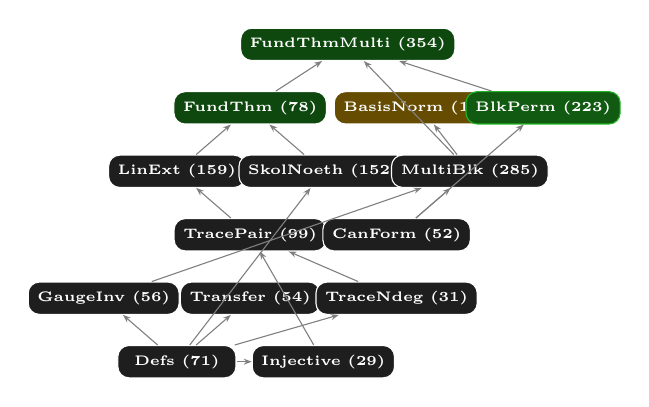
\begin{tikzpicture}[scale=0.62,
  mod/.style={rectangle,rounded corners,draw=white,fill=cardbg,text=white,
              font=\tiny\bfseries,minimum width=1.5cm,minimum height=0.38cm,align=center},
  arr/.style={-{Stealth[scale=0.6]},gray,thin}
]
\node[mod] (defs) at (0,0) {Defs (71)};
\node[mod] (inj) at (3,0) {Injective (29)};
\node[mod] (gauge) at (-1.5,1.3) {GaugeInv (56)};
\node[mod] (trans) at (1.5,1.3) {Transfer (54)};
\node[mod] (tnd) at (4.5,1.3) {TraceNdeg (31)};
\node[mod] (tp) at (1.5,2.6) {TracePair (99)};
\node[mod] (cf) at (4.5,2.6) {CanForm (52)};
\node[mod] (le) at (0,3.9) {LinExt (159)};
\node[mod] (sn) at (3,3.9) {SkolNoeth (152)};
\node[mod] (mb) at (6,3.9) {MultiBlk (285)};
\node[mod,fill=leangreen!40!black] (ft) at (1.5,5.2) {\textbf{FundThm (78)}};
\node[mod,fill=amber!40!black] (bn) at (5,5.2) {BasisNorm (162)};
\node[mod,fill=leangreen!50!black,draw=leangreen] (bp) at (7.5,5.2) {BlkPerm (223)};
\node[mod,fill=leangreen!40!black] (ftm) at (3.5,6.5) {\textbf{FundThmMulti (354)}};
\draw[arr] (defs) -- (gauge);
\draw[arr] (defs) -- (trans);
\draw[arr] (defs) -- (inj);
\draw[arr] (inj) -- (tp);
\draw[arr] (tnd) -- (tp);
\draw[arr] (defs) -- (tnd);
\draw[arr] (tp) -- (le);
\draw[arr] (defs) -- (sn);
\draw[arr] (le) -- (ft);
\draw[arr] (sn) -- (ft);
\draw[arr] (cf) -- (mb);
\draw[arr] (gauge) -- (mb);
\draw[arr] (mb) -- (bn);
\draw[arr] (ft) -- (ftm);
\draw[arr] (mb) -- (ftm);
\draw[arr] (cf) -- (bp);
\draw[arr] (bp) -- (ftm);
\end{tikzpicture}
\end{center}

\column{0.52\textwidth}
\renewcommand{\arraystretch}{1.1}
{\small
\begin{tabular}{lr}
\hline
\textbf{Metric} & \textbf{Value} \\
\hline
Total lines of Lean 4 & 2297 \\
Modules & 15 \\
Axioms / sorries & \textcolor{leangreen}{0 / 0} \\
Mathlib version & v4.27.0 \\
Expansion factor & $\sim$10$\times$ \\
\hline
\end{tabular}}

\vspace{0.3em}
{\small\textbf{Largest modules:}}\\
{\footnotesize
\texttt{FundTheoremMulti} 354\,l,
\texttt{MultiBlock} 285\,l,\\
\texttt{BlockPermutation} \textcolor{leangreen}{223}\,l,
\texttt{BasisNormal} 162\,l,\\
\texttt{LinExt} 159\,l,
\texttt{SkolNoeth} 152\,l}
\end{columns}
\end{frame}

%======================================================================
% SLIDE 26 - Vision
%======================================================================
\begin{frame}{Vision: Towards Formal Quantum Many-Body Theory}
\vspace{-0.5em}
\begin{center}
{\textcolor{leangreen}{\normalsize First machine-checked proof of a foundational theorem in quantum many-body physics}}
\end{center}

\vspace{-0.1em}
\begin{columns}[T]
\column{0.48\textwidth}
{\small\textbf{This opens the door to:}}
\begin{itemize}\itemsep0.05em
  \item {\small\textbf{Verified parent Hamiltonians}}
  \item {\small\textbf{Formal SPT classification} --- $H^2(G,U(1))$}
  \item {\small\textbf{Verified PEPS theorems} --- higher-dim TNs}
  \item {\small\textbf{Formal quantum channels} --- CP maps}
\end{itemize}

\column{0.48\textwidth}
{\small\textbf{Long-term vision:}}
\begin{itemize}\itemsep0.05em
  \item {\small A \textbf{Mathlib-style library} for quantum information}
  \item {\small Bridge algebra/analysis to quantum physics}
  \item {\small Formal verification as \textbf{standard tool} in math-phys}
  \item {\small Community effort: contribute back to Mathlib}
\end{itemize}
\end{columns}

\vspace{0.3em}
\begin{center}
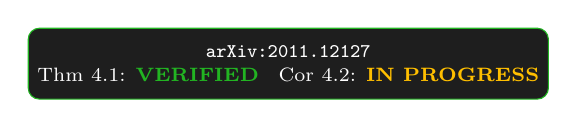
\begin{tikzpicture}
\node[rectangle,rounded corners,draw=leangreen,fill=cardbg,
      text=white,font=\scriptsize,align=center,
      minimum width=3.6cm,minimum height=0.9cm] {
  \texttt{arXiv:2011.12127}\\[0.1em]
  Thm 4.1: \textcolor{leangreen}{\textbf{VERIFIED}}\;\;
  Cor 4.2: \textcolor{amber}{\textbf{IN PROGRESS}}
};
\end{tikzpicture}
\end{center}

\vspace{0.1em}
\begin{center}
{\small\textbf{\textcolor{leangreen}{The future of mathematical physics is formally verified.}}}
\end{center}
\end{frame}

%======================================================================
% SLIDE 27 - Thank You
%======================================================================
\begin{frame}
\begin{center}
\vspace{1em}
\Huge\textbf{\textcolor{leangreen}{Thank You!}}

\vspace{1em}
\LARGE Questions?

\vspace{1.2em}
\large\texttt{github.com/LionSR/MPSLean}

\vspace{0.4em}
\normalsize Built on Lean 4 + Mathlib v4.27.0

\vspace{0.3em}
{\small Reference: Cirac, P\'erez-Garc\'ia, Schuch \& Verstraete\;\;$\cdot$\;\;\texttt{arXiv:2011.12127}}

\vspace{0.8em}
\textcolor{leangreen}{\textbf{2297 lines\quad$\cdot$\quad 15 modules\quad$\cdot$\quad 0 sorries\quad$\cdot$\quad 0 axioms}}
\end{center}
\end{frame}

%======================================================================
%  BACKUP / APPENDIX SLIDES
%======================================================================
\appendix

%======================================================================
% BACKUP 1 - T(1)=1
%======================================================================
\begin{frame}[fragile]{Backup: Proving $T(1)=1$ --- The Nontrivial ``Obvious'' Step}
\vspace{-0.6em}
\begin{columns}[T]
\column{0.46\textwidth}
{\small\textbf{\textcolor{amber}{Why is this needed?}}\\[0.05em]
To apply Skolem--Noether, $T$ must be an \textbf{algebra homomorphism}, requiring $T(1)=1$.
A multiplicative linear map need not preserve~$1$!}

\vspace{0.15em}
{\small\textbf{The argument:}}
\begin{enumerate}\itemsep0.02em
  \item {\small $T$ surjective $\Rightarrow$ pick $x$ with $T(x) = 1$}
  \item {\small $1 \cdot T(1) = T(x) \cdot T(1) = T(x\cdot 1) = T(x) = 1$}
  \item {\small So $T(1) = 1$ \quad\textcolor{leangreen}{\checkmark}}
\end{enumerate}

\vspace{0.12em}
{\small\textbf{Crucially uses:}
\begin{itemize}\itemsep0.01em
  \item \textbf{Surjectivity} (to find $x$)
  \item \textbf{Multiplicativity} ($T(x\cdot 1) = T(x)T(1)$)
\end{itemize}
This is why Step~3 must come \emph{before} Skolem--Noether.}

\column{0.50\textwidth}
{\small\textbf{\textcolor{leangreen}{The Lean proof:}}}
\begin{lstlisting}[basicstyle=\ttfamily\fontsize{5.5}{7}\selectfont\color{white}]
-- From SkolemNoether.lean
have hOne : T 1 = 1 := by
  obtain (*@$\langle$@*)x, hx(*@$\rangle$@*) := hSurj 1
  calc (T 1 : Matrix (Fin D) (Fin D) (*@$\mathbb{C}$@*))
      = 1 * T 1     := (one_mul _).symm
    _ = T x * T 1   := by rw [hx]
    _ = T (x * 1)   := (hMul x 1).symm
    _ = T x          := by rw [mul_one]
    _ = 1            := hx
\end{lstlisting}
\vspace{0.1em}
{\small\textbf{Also needed for \texttt{AlgHom}:}}
\begin{lstlisting}[basicstyle=\ttfamily\fontsize{5.5}{7}\selectfont\color{white}]
commutes' := fun c => by
  simp [Algebra.algebraMap_eq_smul_one,
        hOne]
\end{lstlisting}
\vspace{0.05em}
{\scriptsize\textcolor{dimwhite}{Without \texttt{map\_one'} and \texttt{commutes'}, Lean won't build the \texttt{AlgHom}.}}
\end{columns}
\end{frame}

%======================================================================
% BACKUP 2 - Trace Nondegeneracy
%======================================================================
\begin{frame}[fragile]{Backup: Trace Nondegeneracy --- The Foundational Lemma}
\vspace{-0.6em}
\begin{columns}[T]
\column{0.42\textwidth}
{\small\textbf{\textcolor{amber}{Statement:}}\\[0.05em]
If $\mathrm{tr}(MN) = 0$ for all $N\in M_D(\mathbb{C})$, then $M = 0$.}

\vspace{0.15em}
{\small\textbf{Proof:} Choose $N = E_{ji}$ (single-entry matrix). By cyclicity:}
\vspace{-0.7em}
\[ {\small \mathrm{tr}(E_{ji}\!\cdot\! M) = M_{ij}} \]
\vspace{-0.9em}

{\small So $\mathrm{tr}(MN)=0\ \forall N$ gives $M_{ij}=0$ for all $i,j$.}

\vspace{0.15em}
{\small\textbf{Where this is used:}}
\begin{itemize}\itemsep0.01em
  \item {\scriptsize TracePairing: $\Phi_A$ injective}
  \item {\scriptsize $\to$ LinearExtension: $T$ unique}
  \item {\scriptsize $\to$ Multiplicativity of $T$}
  \item {\scriptsize $\to$ \textbf{Everything downstream!}}
\end{itemize}

\column{0.54\textwidth}
{\small\textbf{\textcolor{leangreen}{Full Lean proof} (TraceNondeg.lean):}}
\begin{lstlisting}[basicstyle=\ttfamily\fontsize{5}{6.5}\selectfont\color{white}]
theorem trace_mul_right_eq_zero_iff
    (M : Matrix n n (*@$\mathbb{C}$@*)) :
    ((*@$\forall$@*) N, trace (M * N) = 0) (*@$\leftrightarrow$@*) M = 0 := by
  classical
  constructor
  (*@$\cdot$@*) intro h
    ext i j
    -- Probe with E_{ji} = Matrix.single j i 1
    have hMN :
      trace (M * Matrix.single j i 1)
        = 0 := h (Matrix.single j i 1)
    -- Use cyclicity: tr(M * E) = tr(E * M)
    have hNM :
      trace (Matrix.single j i 1 * M) = 0 :=
      (trace_mul_comm M
        (Matrix.single j i 1)).symm.trans hMN
    -- Evaluate: tr(E_{ji} * M) = 1 (*@$\bullet$@*) M_{ij}
    have : (1 : (*@$\mathbb{C}$@*)) (*@$\bullet$@*) M i j = 0 := by
      simpa [trace_single_mul] using hNM
    simpa using this
  (*@$\cdot$@*) intro h N
    simp [h]
\end{lstlisting}
\end{columns}
\end{frame}

%======================================================================
% BACKUP 3 - Matrix <-> End Bridge
%======================================================================
\begin{frame}[fragile]{Backup: The Matrix $\leftrightarrow$ End Bridge (``Coercion Hell'')}
\vspace{-0.7em}
{\scriptsize\textbf{Problem:} Mathlib's Skolem--Noether works on $\mathrm{End}_{\mathbb{C}}(\mathbb{C}^n)$, not $M_n(\mathbb{C})$.  Isomorphic $\neq$ definitionally equal!}
\vspace{-0.2em}
\begin{center}
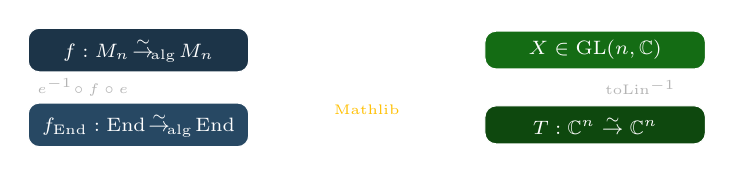
\begin{tikzpicture}[
  box/.style={rectangle,rounded corners,draw=white,text=white,
    font=\scriptsize,minimum width=2.8cm,minimum height=0.45cm,align=center},
  arr/.style={-{Stealth[scale=0.6]},white,thick}
]
\node[box,fill=leanblue!40!black] (f) at (0,0.95) {$f : M_n \!\stackrel{\sim}{\to}_{\!\mathrm{alg}}\! M_n$};
\node[box,fill=leanblue!55!black] (fend) at (0,0) {$f_{\mathrm{End}} : \mathrm{End} \!\stackrel{\sim}{\to}_{\!\mathrm{alg}}\! \mathrm{End}$};
\node[box,fill=leangreen!40!black] (T) at (5.8,0) {$T : \mathbb{C}^n \stackrel{\sim}{\to} \mathbb{C}^n$};
\node[box,fill=leangreen!60!black] (X) at (5.8,0.95) {$X \in \mathrm{GL}(n,\mathbb{C})$};
\draw[arr] (f) -- node[left,font=\tiny,text=dimwhite]{$e^{-1}\!\circ f\circ e$} (fend);
\draw[arr] (fend) -- node[above,font=\tiny,text=amber]{Mathlib} (T);
\draw[arr] (T) -- node[right,font=\tiny,text=dimwhite]{toLin$^{-1}$} (X);
\end{tikzpicture}
\end{center}

\vspace{-0.35em}
\begin{columns}[T]
\column{0.46\textwidth}
{\scriptsize\textbf{Steps 1--3:} Transport, apply, convert back:}
\begin{lstlisting}[basicstyle=\ttfamily\fontsize{4.5}{5.5}\selectfont\color{white}]
-- Step 1: transport to End
let e := Matrix.toLinAlgEquiv'
let fEnd := e.symm.trans (f.trans e)
-- Step 2: apply Mathlib's Skolem-Noether
obtain (*@$\langle$@*)T, hT(*@$\rangle$@*) :=
  AlgEquiv.eq_linearEquivConjAlgEquiv
    (f := fEnd)
-- Step 3: convert back to GL
let X : GL n (*@$\mathbb{C}$@*) :=
  (GeneralLinearGroup.toLin).symm
    (ofLinearEquiv T)
\end{lstlisting}

\column{0.50\textwidth}
{\scriptsize\textbf{Step 4 (hard):} Prove $e(X) = T$ as linear maps:}
\begin{lstlisting}[basicstyle=\ttfamily\fontsize{4.5}{5.5}\selectfont\color{white}]
-- Chase: Units.mapEquiv, coe_mapEquiv,
-- GeneralLinearGroup.toLin
have hX_lin :
  e (X : Matrix n n (*@$\mathbb{C}$@*)) = (T : ...) := ...
have hX_lin_inv :
  e ((X(*@$^{-1}$@*) : GL n (*@$\mathbb{C}$@*)) : Matrix ..)
    = (T.symm : ...) := ...
\end{lstlisting}
\vspace{0.01em}
{\scriptsize\textbf{Step 5:} Final \texttt{calc}:}
\begin{lstlisting}[basicstyle=\ttfamily\fontsize{4.5}{5.5}\selectfont\color{white}]
calc e (f M)
    = fEnd (e M)         := by simp
  _ = T (*@$\circ$@*) (e M) (*@$\circ$@*) T.symm := ...
  _ = e (X * M * X(*@$^{-1}$@*))   := by
        rw [hX_lin, hX_lin_inv]; simp
\end{lstlisting}
\vspace{0.02em}
{\scriptsize\textcolor{amber}{\textbf{152 lines}} for this bridge alone!}
\end{columns}
\end{frame}

%======================================================================
% BACKUP 4 - Injectivity Definitions
%======================================================================
\begin{frame}[fragile]{Backup: Injectivity --- Algebraic vs.\ Physical Definitions}
\vspace{-0.5em}
\begin{columns}[T]
\column{0.52\textwidth}
{\small Three notions in the MPS literature:}

\vspace{0.15em}
{\small\textbf{1.\ Linear independence} (weakest) ---
$\{A^i\}$ linearly independent.  Requires $d \leq D^2$. \emph{Not sufficient.}}

\vspace{0.1em}
{\small\textbf{2.\ Algebraic injectivity} \textcolor{leangreen}{$\boldsymbol{\leftarrow}$ ours} ---
$\mathrm{span}_{\mathbb{C}}\{A^i\} = M_D(\mathbb{C})$.
Requires $d \geq D^2$.}

\vspace{0.1em}
{\small\textbf{3.\ CP-map injectivity} (physical) ---
$E_A(X) = \sum_i A^i X (A^i)^\dagger$ has unique full-rank fixed point.}

\vspace{0.15em}
{\small\textbf{Relationships:}
$(2) \!\Rightarrow\! (1)$: spanning $\Rightarrow$ indep.
$(2) \!\Rightarrow\! (3)$: quantum Wielandt.
$(3) \!\Rightarrow\! (2)$: for \textbf{normal} MPS after blocking.}

\column{0.44\textwidth}
{\small\textbf{\textcolor{leangreen}{Why we chose (2):}}}
\begin{itemize}\itemsep0.02em
  \item {\small Purely algebraic: \texttt{Submodule.span}}
  \item {\small No CP maps or Perron--Frobenius}
  \item {\small Makes $\ker T$ argument work}
\end{itemize}

\vspace{0.15em}
{\small\textbf{The Lean definition:}}
\begin{lstlisting}[basicstyle=\ttfamily\fontsize{5.5}{7}\selectfont\color{white}]
def IsInjective
    (A : MPSTensor d D) :=
  Submodule.span (*@$\mathbb{C}$@*)
    (Set.range A) = (*@$\top$@*)
\end{lstlisting}

\vspace{0.1em}
{\small\textbf{\textcolor{softred}{What (3) would need:}}}
\begin{itemize}\itemsep0.01em
  \item {\scriptsize Perron--Frobenius for positive maps}
  \item {\scriptsize Spectral theory (partial in Mathlib)}
  \item {\scriptsize $C^*$-algebra structure}
\end{itemize}
\vspace{0.05em}
{\scriptsize We \emph{do} define $E_A$ in \texttt{Transfer.lean} and prove positivity, but can't access spectral properties.}
\end{columns}
\end{frame}

%======================================================================
% BACKUP 5 - MPV Decomposition
%======================================================================
\begin{frame}[fragile]{Backup: MPV Decomposition --- The Full Computation}
\vspace{-0.6em}
{\small\textbf{Goal:} $\mathrm{mpv}(C.\mathrm{toTensor}, \sigma) = \sum_{k=1}^{r} \mu_k^N \cdot \mathrm{mpv}(A_k, \sigma)$
\quad---\quad ``one line in physics'', \textbf{six formal steps}:}
\vspace{-0.4em}
{\scriptsize
\begin{align*}
\mathrm{mpv}(C, \sigma) &= \mathrm{tr}\!\big(\underbrace{C^{i_1}\!\cdots C^{i_N}}_{\texttt{evalWord}}\big) && \text{\textcolor{dimwhite}{[definition]}}\\[-3pt]
&= \mathrm{tr}\!\big(\mathrm{reindex}_e(\mathrm{BD}^{i_1}\!\cdots \mathrm{BD}^{i_N})\big) && \text{\textcolor{dimwhite}{[\texttt{evalWord\_reindex}]}}\\[-3pt]
&= \mathrm{tr}\!\big(\mathrm{BD}^{i_1}\!\cdots \mathrm{BD}^{i_N}\big) && \text{\textcolor{dimwhite}{[\texttt{trace\_reindex}]}}\\[-3pt]
&= \mathrm{tr}\!\big(\mathrm{blockDiag}(\mu_k^N A_k^{i_1}\!\cdots A_k^{i_N})\big) && \text{\textcolor{dimwhite}{[\texttt{evalWord\_blockDiag'\_smul}]}}\\[-3pt]
&= \textstyle\sum_k \mathrm{tr}\!\big(\mu_k^N A_k^{i_1}\!\cdots A_k^{i_N}\big) && \text{\textcolor{dimwhite}{[\texttt{trace\_blockDiagonal'}]}}\\[-3pt]
&= \textstyle\sum_k \mu_k^N \cdot \mathrm{mpv}(A_k, \sigma) && \text{\textcolor{dimwhite}{[\texttt{trace\_smul}]}}
\end{align*}
}

\vspace{-0.8em}
\begin{columns}[T]
\column{0.48\textwidth}
{\small\textbf{The $\Sigma$-type trick:}}\\[0.05em]
{\scriptsize Block-diagonal uses index type
$\bigsqcup_k \mathrm{Fin}(D_k)$, not $\mathrm{Fin}(\sum_k D_k)$.
Multiplication is \emph{definitional} via \texttt{blockDiagonal'\_mul} --- no sub-range arithmetic.
Reindex to $\mathrm{Fin}(\sum D_k)$ only at the end, then immediately remove via \texttt{trace\_reindex}.}

\vspace{0.1em}
{\small\textbf{\textcolor{leangreen}{Design payoff:}} Avoids $>$100 lines of \texttt{Fin} lemmas.}

\column{0.48\textwidth}
{\small\textbf{Why 285 lines?}}\\[0.05em]
{\scriptsize Each step: separate lemma, induction on word length.

\vspace{0.05em}
\renewcommand{\arraystretch}{0.95}
\begin{tabular}{lr}
\texttt{evalWord\_blockDiagonal'} & 20\,l \\
\texttt{evalWord\_blockDiag'\_smul} & 35\,l \\
\texttt{trace\_reindex} & 12\,l \\
\texttt{evalWord\_reindex} & 30\,l \\
\texttt{mpv\_toTensor\_eq\_sum} & 65\,l \\
\texttt{GaugePhaseEquiv.prop..} & 55\,l \\
\end{tabular}

\vspace{0.05em}
Scalars accumulate via \texttt{smul\_smul}, \texttt{pow\_succ'}.}
\end{columns}
\end{frame}

\end{document}